\documentclass[]{article}
\usepackage{lmodern}
\usepackage{amssymb,amsmath}
\usepackage{ifxetex,ifluatex}
\usepackage{fixltx2e} % provides \textsubscript
\ifnum 0\ifxetex 1\fi\ifluatex 1\fi=0 % if pdftex
  \usepackage[T1]{fontenc}
  \usepackage[utf8]{inputenc}
\else % if luatex or xelatex
  \ifxetex
    \usepackage{mathspec}
    \usepackage{xltxtra,xunicode}
  \else
    \usepackage{fontspec}
  \fi
  \defaultfontfeatures{Mapping=tex-text,Scale=MatchLowercase}
  \newcommand{\euro}{€}
\fi
% use upquote if available, for straight quotes in verbatim environments
\IfFileExists{upquote.sty}{\usepackage{upquote}}{}
% use microtype if available
\IfFileExists{microtype.sty}{%
\usepackage{microtype}
\UseMicrotypeSet[protrusion]{basicmath} % disable protrusion for tt fonts
}{}
\usepackage[margin=1in]{geometry}
\usepackage{longtable,booktabs}
\usepackage{graphicx}
\makeatletter
\def\maxwidth{\ifdim\Gin@nat@width>\linewidth\linewidth\else\Gin@nat@width\fi}
\def\maxheight{\ifdim\Gin@nat@height>\textheight\textheight\else\Gin@nat@height\fi}
\makeatother
% Scale images if necessary, so that they will not overflow the page
% margins by default, and it is still possible to overwrite the defaults
% using explicit options in \includegraphics[width, height, ...]{}
\setkeys{Gin}{width=\maxwidth,height=\maxheight,keepaspectratio}
\ifxetex
  \usepackage[setpagesize=false, % page size defined by xetex
              unicode=false, % unicode breaks when used with xetex
              xetex]{hyperref}
\else
  \usepackage[unicode=true]{hyperref}
\fi
\hypersetup{breaklinks=true,
            bookmarks=true,
            pdfauthor={Daniel Brooks (daniel.brooks@spsmail.cuny.edu), Daniel Fanelli (daniel.fanelli@spsmail.cuny.edu), Christopher Fenton (christopher.fenton@spsmail.cuny.edu), James Hamski (james.hamski@spsmail.cuny.edu), Youqing Xiang (youqing.xiang@spsmail.cuny.edu)},
            pdftitle={Using Losistic Regression to Predict Boston Neighborhood Crime Levels},
            colorlinks=true,
            citecolor=blue,
            urlcolor=blue,
            linkcolor=magenta,
            pdfborder={0 0 0}}
\urlstyle{same}  % don't use monospace font for urls
\setlength{\parindent}{0pt}
\setlength{\parskip}{6pt plus 2pt minus 1pt}
\setlength{\emergencystretch}{3em}  % prevent overfull lines
\setcounter{secnumdepth}{5}

%%% Use protect on footnotes to avoid problems with footnotes in titles
\let\rmarkdownfootnote\footnote%
\def\footnote{\protect\rmarkdownfootnote}

%%% Change title format to be more compact
\usepackage{titling}

% Create subtitle command for use in maketitle
\newcommand{\subtitle}[1]{
  \posttitle{
    \begin{center}\large#1\end{center}
    }
}

\setlength{\droptitle}{-2em}
  \title{Using Losistic Regression to Predict Boston Neighborhood Crime Levels}
  \pretitle{\vspace{\droptitle}\centering\huge}
  \posttitle{\par}
  \author{Daniel Brooks
(\href{mailto:daniel.brooks@spsmail.cuny.edu}{\nolinkurl{daniel.brooks@spsmail.cuny.edu}}),
Daniel Fanelli
(\href{mailto:daniel.fanelli@spsmail.cuny.edu}{\nolinkurl{daniel.fanelli@spsmail.cuny.edu}}),
Christopher Fenton
(\href{mailto:christopher.fenton@spsmail.cuny.edu}{\nolinkurl{christopher.fenton@spsmail.cuny.edu}}),
James Hamski
(\href{mailto:james.hamski@spsmail.cuny.edu}{\nolinkurl{james.hamski@spsmail.cuny.edu}}),
Youqing Xiang
(\href{mailto:youqing.xiang@spsmail.cuny.edu}{\nolinkurl{youqing.xiang@spsmail.cuny.edu}})}
  \preauthor{\centering\large\emph}
  \postauthor{\par}
  \predate{\centering\large\emph}
  \postdate{\par}
  \date{7/3/2016}



\begin{document}

\maketitle


The purpose of this analysis is to build a logistic regression model
that will predict whether a particular neighborhood in Boston is above
or below the median crime level for the city.

Our dataset includes information on 466 Boston neighborhoods. Each
neighborhood has 13 potential predictor variables, and 1 response
variable. The response variable is ``target'', which is ``1'' if the
neighbhorhood is above the city's median crime level, and 0 if not.

\section{Data Exploration}\label{data-exploration}

The first thing we checked for was if there was missing data in any of
the variables. There was no missing data.

Of the 13 predictor variables, 12 were numeric and 1 was caterogical.
The categorical data would need to be converted in order to be
approrpriately used in a generalized linear model.

We also examined the distribution of the response variable,
\texttt{target}. 229 neighborhoods were marked with a 1, thus above the
median crime level, and 237 were not. The fact that the two numbers were
not within 1 of each other implies that some neighbohood data was not
included. However, the split was roughly even, allowing us to proceed.

\textbf{Figure 1.1}

\begin{verbatim}
##        zn             indus             chas              nox        
##  Min.   :  0.00   Min.   : 0.460   Min.   :0.00000   Min.   :0.3890  
##  1st Qu.:  0.00   1st Qu.: 5.145   1st Qu.:0.00000   1st Qu.:0.4480  
##  Median :  0.00   Median : 9.690   Median :0.00000   Median :0.5380  
##  Mean   : 11.58   Mean   :11.105   Mean   :0.07082   Mean   :0.5543  
##  3rd Qu.: 16.25   3rd Qu.:18.100   3rd Qu.:0.00000   3rd Qu.:0.6240  
##  Max.   :100.00   Max.   :27.740   Max.   :1.00000   Max.   :0.8710  
##        rm             age              dis              rad       
##  Min.   :3.863   Min.   :  2.90   Min.   : 1.130   Min.   : 1.00  
##  1st Qu.:5.887   1st Qu.: 43.88   1st Qu.: 2.101   1st Qu.: 4.00  
##  Median :6.210   Median : 77.15   Median : 3.191   Median : 5.00  
##  Mean   :6.291   Mean   : 68.37   Mean   : 3.796   Mean   : 9.53  
##  3rd Qu.:6.630   3rd Qu.: 94.10   3rd Qu.: 5.215   3rd Qu.:24.00  
##  Max.   :8.780   Max.   :100.00   Max.   :12.127   Max.   :24.00  
##       tax           ptratio         black            lstat       
##  Min.   :187.0   Min.   :12.6   Min.   :  0.32   Min.   : 1.730  
##  1st Qu.:281.0   1st Qu.:16.9   1st Qu.:375.61   1st Qu.: 7.043  
##  Median :334.5   Median :18.9   Median :391.34   Median :11.350  
##  Mean   :409.5   Mean   :18.4   Mean   :357.12   Mean   :12.631  
##  3rd Qu.:666.0   3rd Qu.:20.2   3rd Qu.:396.24   3rd Qu.:16.930  
##  Max.   :711.0   Max.   :22.0   Max.   :396.90   Max.   :37.970  
##       medv           target      
##  Min.   : 5.00   Min.   :0.0000  
##  1st Qu.:17.02   1st Qu.:0.0000  
##  Median :21.20   Median :0.0000  
##  Mean   :22.59   Mean   :0.4914  
##  3rd Qu.:25.00   3rd Qu.:1.0000  
##  Max.   :50.00   Max.   :1.0000
\end{verbatim}

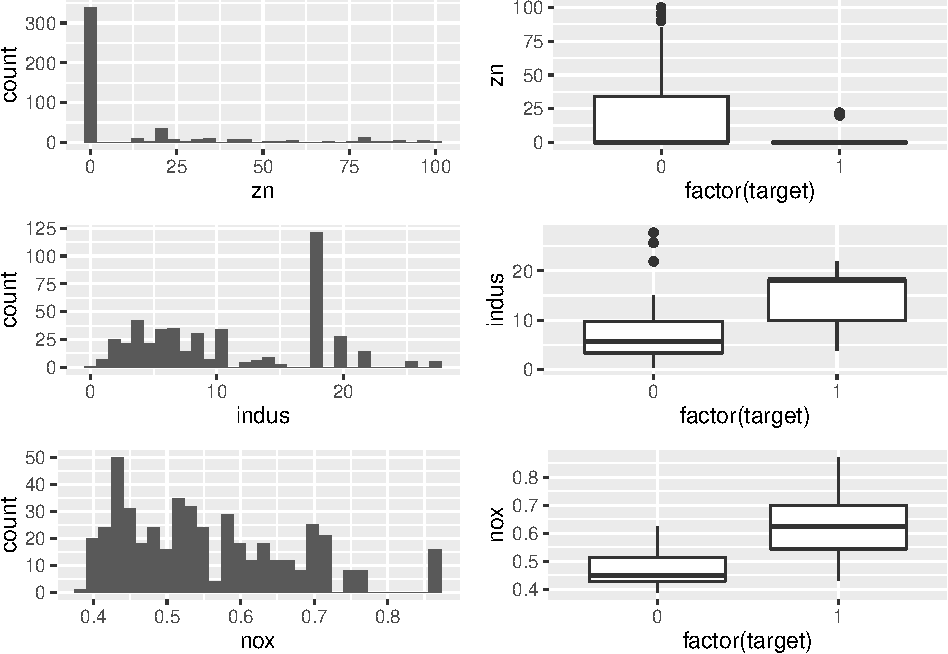
\includegraphics{HW3_Final_files/figure-latex/unnamed-chunk-2-1.pdf}
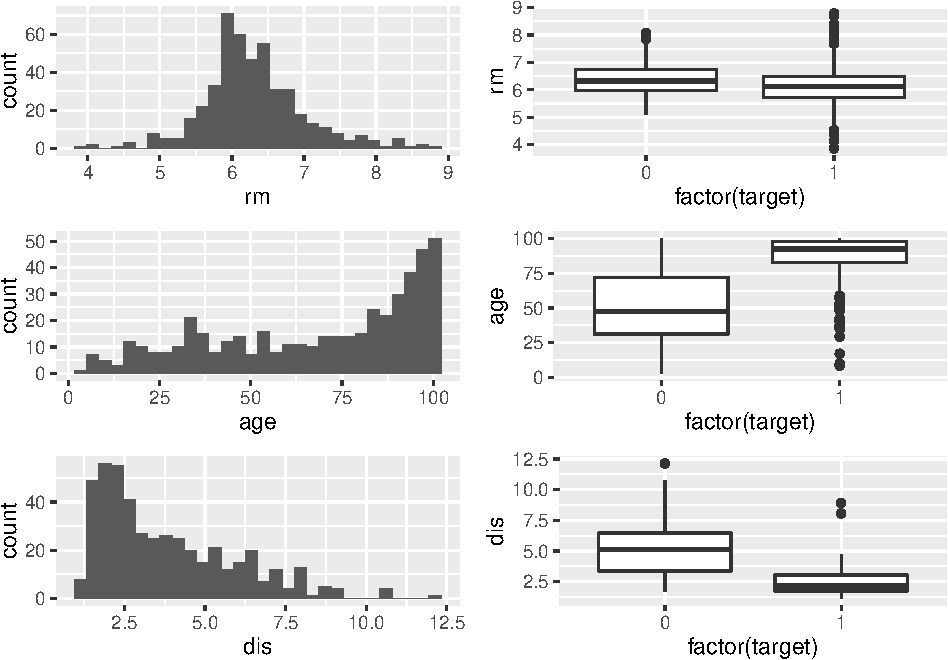
\includegraphics{HW3_Final_files/figure-latex/unnamed-chunk-2-2.pdf}
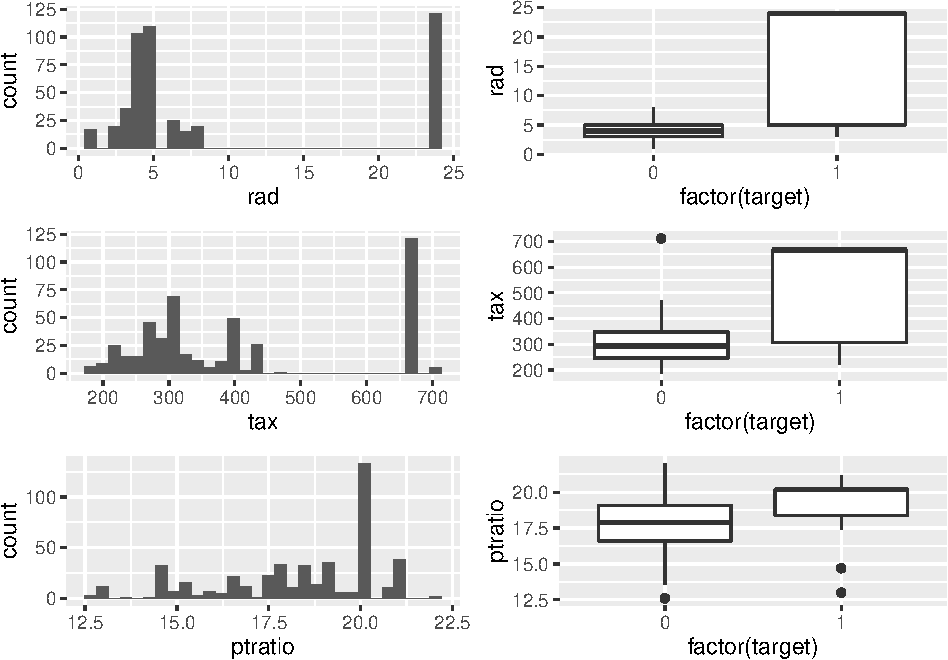
\includegraphics{HW3_Final_files/figure-latex/unnamed-chunk-2-3.pdf}
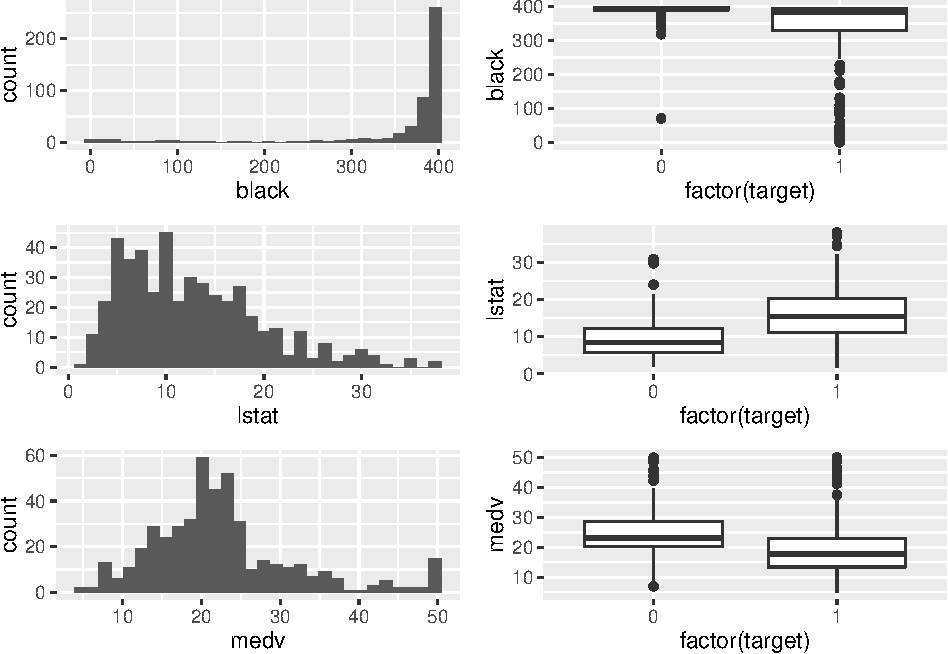
\includegraphics{HW3_Final_files/figure-latex/unnamed-chunk-2-4.pdf}

Using histograms of variables and boxplots of variables grouped by
predictor (Figure 1.1), we could see some outliers that may need to be
dealt with. Also, correlations with the response variable
(\texttt{target}) showed that variables such as \texttt{zn},
\texttt{indus}, \texttt{dis} and \texttt{rad} may have more potential as
predictor variables while \texttt{chas} and \texttt{rm} may not be as
useful.

\pagebreak  

\textbf{Figure
1.2}\\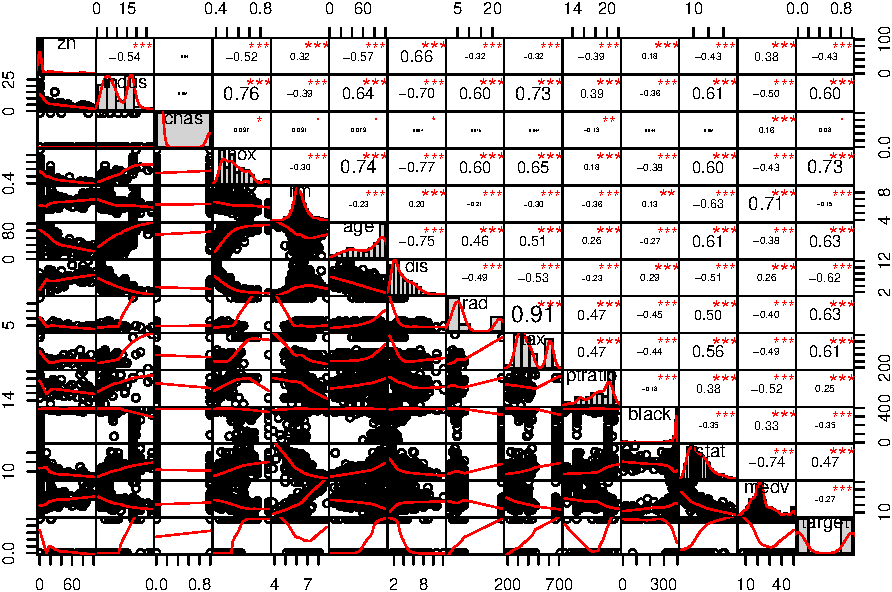
\includegraphics{HW3_Final_files/figure-latex/unnamed-chunk-4-1.pdf}

Figure 1.2 shows that every variable other than adjancency to the
Charles river has correlation significance level of .001 with our
response variable, \texttt{target}. This graph also shows that
multicollinearity is something that will have to be dealt with in this
model. Principal component analysis could be useful to mitigate this.

The fact that the predictor variables show a high degree of correlation
with each other makes intuitive sense. Most variables relate to a notion
of ``desirability'', which would hypothetically have significant impacts
on other variables.

For instance, one might suppose that a high degree of industrial real
estate in a neighborhood would have a negative effect on real estate
values. One might than hypothesize that a neighborhood with lower median
real estate values would be more highly susceptible to higher than usual
crime.

At least in the provided dataset, there are strong correlations that
bear out both of those hypotheses. \texttt{Indus}, which describes the
proportion of non-retail businesses in a neighborhood, is negatively
correlated by a factor of -.49617 with \texttt{Medv}, the median value
of owner occupied homes; \texttt{Medv} is negative correlated (-.27)
with higher than normal crime rates.

\section{Data Preparation}\label{data-preparation}

We used two separate approaches to preparing the data. One approach
dealt with each variable separately, while the second approach
normalized all variables.

\subsection{Individual Variable Preparation
Approach}\label{individual-variable-preparation-approach}

This approach looked at each variable independently of the others.

\subsubsection{zn}\label{zn}

\textbf{Figure
2.1}\\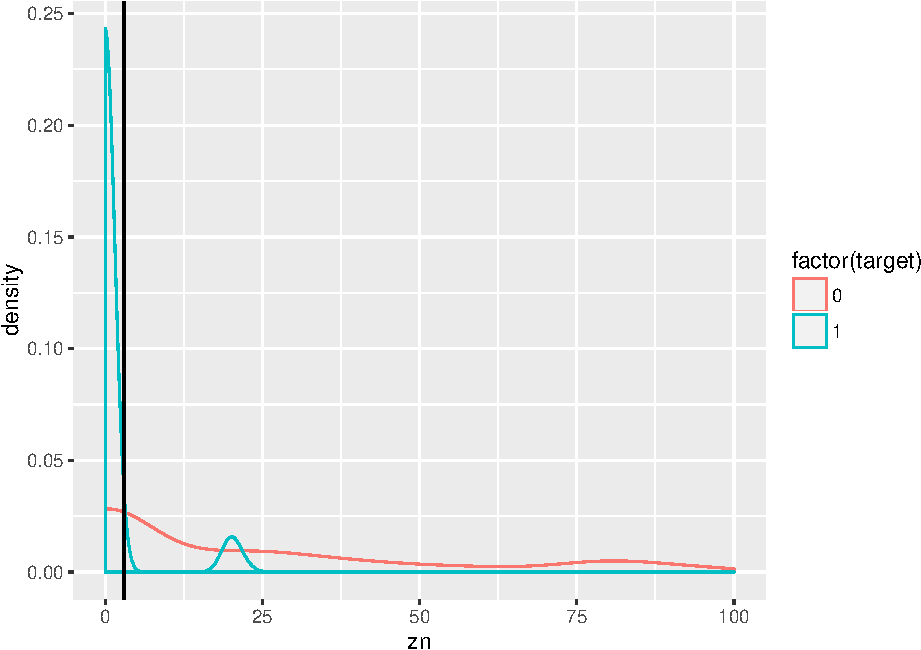
\includegraphics{HW3_Final_files/figure-latex/unnamed-chunk-5-1.pdf}

\begin{longtable}[c]{@{}ccc@{}}
\toprule
znN & Target & Freq\tabularnewline
\midrule
\endhead
0 & 0 & 125\tabularnewline
1 & 0 & 112\tabularnewline
0 & 1 & 214\tabularnewline
1 & 1 & 15\tabularnewline
\bottomrule
\end{longtable}

Using Figure 2.1, we decided to transform the numeric \texttt{z}
variable to a derived categorical variable called \texttt{znN}. For this
new \texttt{znN} variable, \emph{1} means more than 3\% of residential
land zoned for large lots (over 25000 square feet), and \emph{0} means
less than or equal to 3\% of residential land zoned for large lots (over
25000 square feet).

\subsubsection{indus}\label{indus}

Each observation in the dataset is for a different Boston area
neighborhood. This means the data are somewhat arbitrarily binned by
geography - the area that is considered a neighborhood is influenced by
historical factors. For instance, we see high-value outliers in the
\texttt{indus} variable because historic land-use and zoning laws mean
that non-retail business use is concentrated in specific industrial
areas. In order to remove these potential leverage points, we removed
neighborhoods with indus values above 20. However, we do not consider
this to be invalid data.

\pagebreak  

\textbf{Figure 2.3}

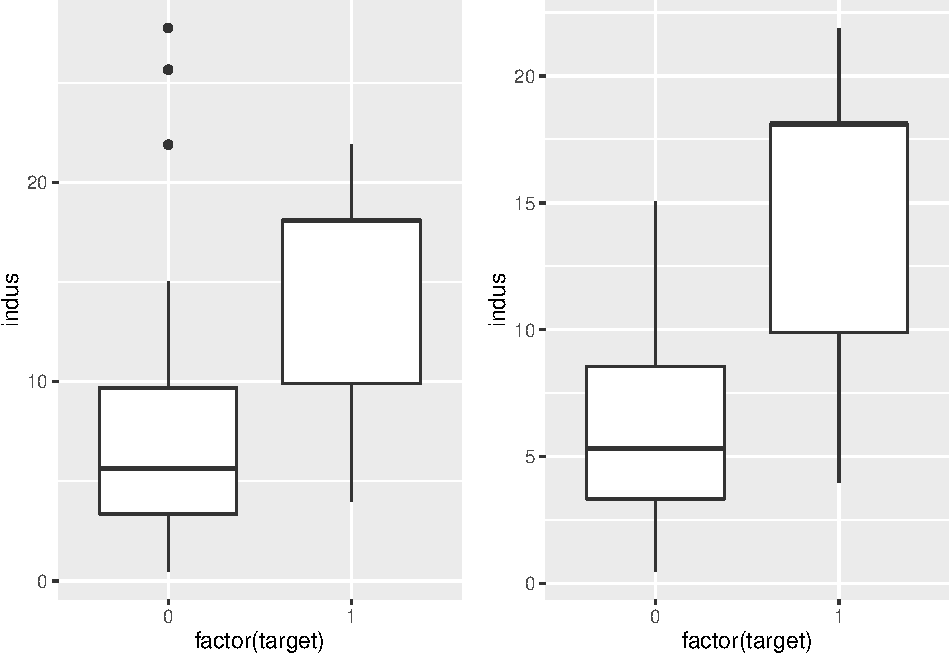
\includegraphics{HW3_Final_files/figure-latex/unnamed-chunk-6-1.pdf}

For \texttt{indus}, we removed observations where \texttt{indus} was
greater than 20 and \texttt{target} was 0.

\subsubsection{dis}\label{dis}

\textbf{Figure
2.4}\\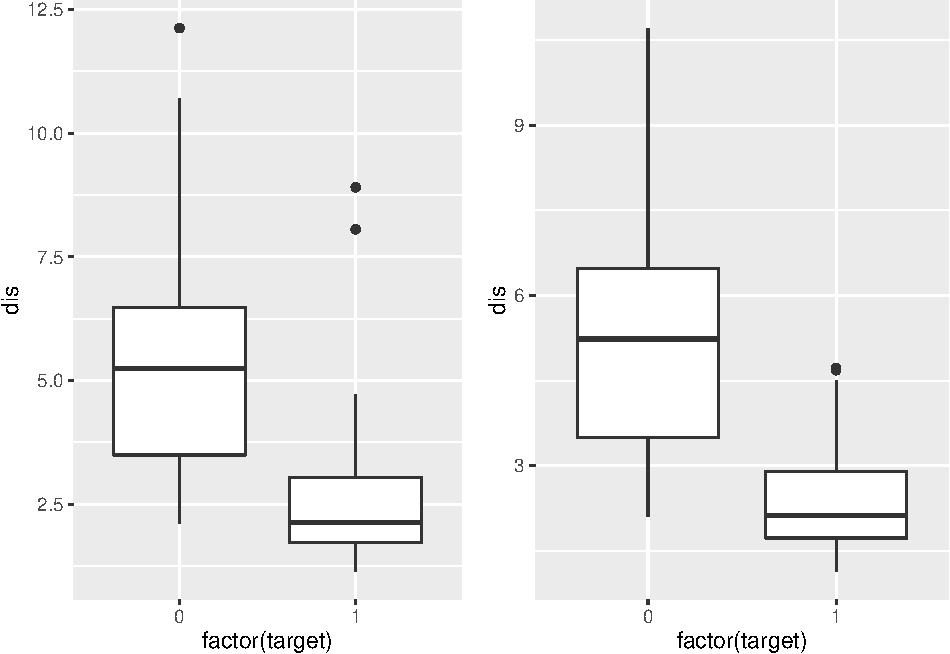
\includegraphics{HW3_Final_files/figure-latex/unnamed-chunk-7-1.pdf}

We removed observations where \texttt{dis} was greater than 11 and
\texttt{target} was 0, and observations where \texttt{dis} was greater
than 7.5 and \texttt{target} was 1.

\subsubsection{7. rad}\label{rad}

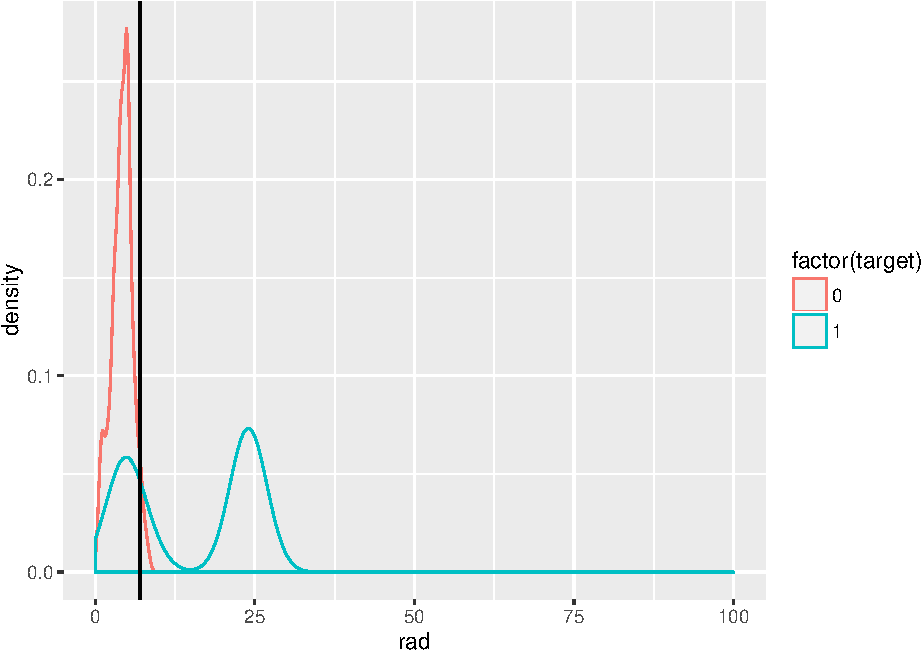
\includegraphics{HW3_Final_files/figure-latex/unnamed-chunk-8-1.pdf}

\begin{longtable}[c]{@{}llr@{}}
\toprule
radN & Target & Freq\tabularnewline
\midrule
\endhead
0 & 0 & 221\tabularnewline
1 & 0 & 4\tabularnewline
0 & 1 & 90\tabularnewline
1 & 1 & 137\tabularnewline
\bottomrule
\end{longtable}

Here we applied the same method as \texttt{zn}. We set up a new variable
called \texttt{radN}, where \emph{1} means index of accessibility to
radial highways was greater than 7 and \emph{0} means index of
accessibility to radial highways was less than or equal to 7.

\subsubsection{Summary}\label{summary}

Under our first approach, we removed 14 rows and added 2 new variables:
\texttt{znN} and \texttt{radN}.

\subsection{Normalization Approach}\label{normalization-approach}

Since the variables were on a variety of scales, we created a dataset of
centered (predictor variable mean subtracted from each observation) and
scaled (each observation divided by the predictor variable's standard
deviation) data. The two datasets are distinguished as `non-normalized'
and `normalized' below, with the latter having been centered and scaled
using R's `scale' function.

\section{Build Models}\label{build-models}

Since the evaluation data set did not include the response variable, we
were not able to use it to cross validate our models. Instead, we split
the training data on a 70-30 training/testing split to evaluate our
models.

\subsection{Model 1: Non-normalized
Baseline}\label{model-1-non-normalized-baseline}

This model used the non-normalized original variables. It utilized the
probit for the link function. The model began with all the original
values, and via backwards selection removed the \texttt{zn},
\texttt{chas}, \texttt{rm}, \texttt{dis}, and \texttt{black} variables.

\begin{verbatim}
## 
## Call:
## glm(formula = target ~ indus + nox + age + rad + tax + ptratio + 
##     lstat + medv, family = binomial(link = "probit"), data = training)
## 
## Deviance Residuals: 
##    Min      1Q  Median      3Q     Max  
## -2.343  -0.026   0.000   0.000   2.882  
## 
## Coefficients:
##               Estimate Std. Error z value Pr(>|z|)    
## (Intercept) -24.171357   4.325079  -5.589 2.29e-08 ***
## indus         0.134991   0.060490   2.232 0.025639 *  
## nox          28.874385   5.510981   5.239 1.61e-07 ***
## age           0.015291   0.007279   2.101 0.035654 *  
## rad           0.491912   0.136730   3.598 0.000321 ***
## tax          -0.017047   0.004355  -3.914 9.07e-05 ***
## ptratio       0.344176   0.103985   3.310 0.000933 ***
## lstat         0.099590   0.035125   2.835 0.004579 ** 
## medv          0.079078   0.029423   2.688 0.007196 ** 
## ---
## Signif. codes:  0 '***' 0.001 '**' 0.01 '*' 0.05 '.' 0.1 ' ' 1
## 
## (Dispersion parameter for binomial family taken to be 1)
## 
##     Null deviance: 438.75  on 316  degrees of freedom
## Residual deviance: 102.98  on 308  degrees of freedom
## AIC: 120.98
## 
## Number of Fisher Scoring iterations: 11
\end{verbatim}

From the output, the model is as follows:

the log odds of \texttt{target} = -24.17 + 0.135 \texttt{indus} + 28.874
\texttt{nox} + 0.015 \texttt{age} + 0.492 \texttt{rad} - 0.017
\texttt{tax} + 0.344 \texttt{ptratio} + 0.1 \texttt{lstat} + 0.079
\texttt{medv}

We can see that \texttt{indus}, \texttt{nox}, \texttt{age},
\texttt{rad}, \texttt{ptratio}, \texttt{lstat}, and \texttt{medv} have
positive effects on \texttt{target}, but \texttt{tax} has a negative
effect on \texttt{target}.

For this model, the most unexpected result is that \texttt{medv} (median
value of owner-occupied homes in \$1000s) has a positive effect on
crime. And if we go back to check figure 1.2, we saw the weak negative
correlationship (-0.27) between \texttt{medv} and \texttt{target}. Since
this model includes \texttt{indus}, \texttt{nox}, \texttt{age},
\texttt{rad}, \texttt{ptratio}, \texttt{lstat}, \texttt{medv} and
\texttt{tax}, \textbf{multicollinearity} could be the root cause.

\subsection{Model 2: Non-normalized with derived
variables}\label{model-2-non-normalized-with-derived-variables}

This model also used backward selection on the non-normalized variables
and the probit for the link function, but instead used the derived
variables from part 2, instead of their original counterparts.

\begin{verbatim}
## 
## Call:
## glm(formula = target ~ nox + tax + lstat + radN, family = binomial(link = "probit"), 
##     data = training)
## 
## Deviance Residuals: 
##      Min        1Q    Median        3Q       Max  
## -2.32446  -0.04097   0.00000   0.02465   2.62981  
## 
## Coefficients:
##               Estimate Std. Error z value Pr(>|z|)    
## (Intercept) -16.708448   2.552283  -6.546 5.89e-11 ***
## nox          32.430637   5.246318   6.182 6.35e-10 ***
## tax          -0.005576   0.002087  -2.672  0.00754 ** 
## lstat         0.080376   0.027954   2.875  0.00404 ** 
## radN1         2.932473   0.556149   5.273 1.34e-07 ***
## ---
## Signif. codes:  0 '***' 0.001 '**' 0.01 '*' 0.05 '.' 0.1 ' ' 1
## 
## (Dispersion parameter for binomial family taken to be 1)
## 
##     Null deviance: 438.75  on 316  degrees of freedom
## Residual deviance: 107.01  on 312  degrees of freedom
## AIC: 117.01
## 
## Number of Fisher Scoring iterations: 9
\end{verbatim}

From the output, the model is as follows:

the log odds of \texttt{target} = -16.71 + 32.43 \texttt{nox} - 0.006
\texttt{tax} + 0.08 \texttt{lstat} + 2.93 radN1

We can see that \texttt{nox} and \texttt{lstat} have positive effects on
the log odds of \texttt{target}, but \texttt{tax} has a negative effect
on the log odds of \texttt{target}. In addition, when radN equals to 1,
the log odds of \texttt{target} increases by 2.93.

This model only include 4 variables and we transformed \texttt{rad} to
categorical variable \texttt{radN}, so \textbf{multicollinearity} became
less of an issue to us. Although we saw a positve correlation between
\texttt{tax} and \texttt{target} in figure 1.2, both Model 1 and Model 2
show that \texttt{tax} has a negative yet weak effect on the log odds of
\texttt{target}, which fits our intuition.

\subsection{Model 3: Principle Component
Analysis}\label{model-3-principle-component-analysis}

For this model, we used an orthogonal transformation to convert our
variables (normalization applied to all variables) into a set of values
of linearly uncorrelated variables, which is called principal
components. And then we chose the first two principal components that
account for around 95\% proportion of variance in the data. Finally, we
used those chosen principal components to build a logistic regression
model.

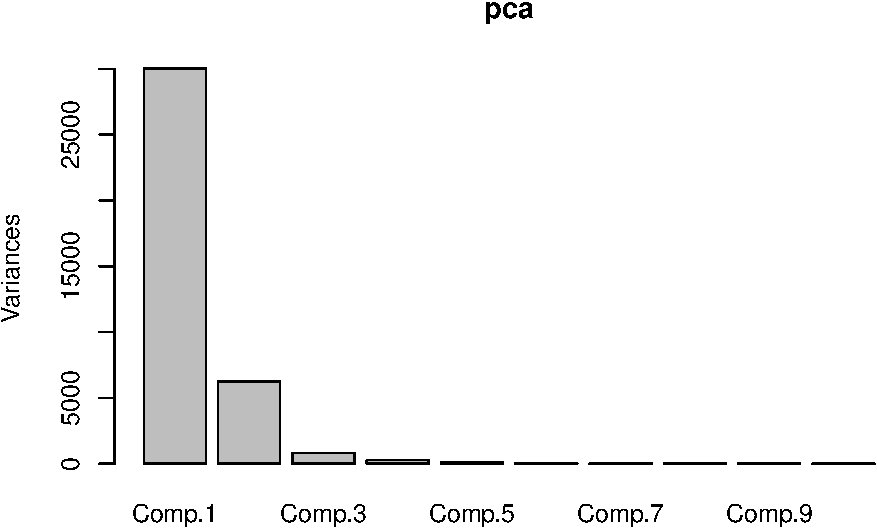
\includegraphics{HW3_Final_files/figure-latex/unnamed-chunk-13-1.pdf}

\begin{verbatim}
##   target      Comp.1     Comp.2
## 1      1    7.982215  -10.79214
## 2      1   14.663799  -36.79382
## 3      1 -237.185595 -109.13296
## 4      0  115.531924   17.45648
## 5      0  214.333148   31.11811
## 6      0   35.789981  -29.36113
\end{verbatim}

\begin{verbatim}
## 
## Call:
## glm(formula = target ~ ., data = training_pca)
## 
## Deviance Residuals: 
##      Min        1Q    Median        3Q       Max  
## -0.59191  -0.27404  -0.10935   0.04818   0.83770  
## 
## Coefficients:
##               Estimate Std. Error t value Pr(>|t|)    
## (Intercept)  0.5116620  0.0217455  23.530   <2e-16 ***
## Comp.1      -0.0018248  0.0001246 -14.639   <2e-16 ***
## Comp.2      -0.0001726  0.0002618  -0.659     0.51    
## ---
## Signif. codes:  0 '***' 0.001 '**' 0.01 '*' 0.05 '.' 0.1 ' ' 1
## 
## (Dispersion parameter for gaussian family taken to be 0.1496637)
## 
##     Null deviance: 79.073  on 316  degrees of freedom
## Residual deviance: 46.994  on 314  degrees of freedom
## AIC: 302.49
## 
## Number of Fisher Scoring iterations: 2
\end{verbatim}

From the output, the formula we got was the following:

the log odds of \texttt{target} = 0.512 - 0.00182 \texttt{Comp.1} -
0.00017 \texttt{Comp.2}

For this model, since we did an orthogonal transformation of variables,
\textbf{multicollinearity} was no longer an issue. Both principal
components have negative effects on the log odds of \texttt{target}. And
we only chose two principal components, so we keep the model as is, even
though the p value of \texttt{Comp.2} is not significant.

\subsection{Model 4: Normalized Backward
Selection}\label{model-4-normalized-backward-selection}

This model used the normalized data, the logit in the link function, and
used backward selection using R's step() function with the backward
option to arive at the below model. Insignificant variables (those with
a P value \textgreater{} .05) were discarded.

\begin{verbatim}
## 
## Call:
## glm(formula = target ~ nox + age + rad + tax + ptratio + black + 
##     medv, family = binomial, data = training_norm)
## 
## Deviance Residuals: 
##      Min        1Q    Median        3Q       Max  
## -1.85486  -0.18466  -0.01769   0.00474   2.84168  
## 
## Coefficients:
##             Estimate Std. Error z value Pr(>|z|)    
## (Intercept)   3.7989     0.9758   3.893 9.90e-05 ***
## nox           3.7313     0.6959   5.362 8.23e-08 ***
## age           0.7877     0.3430   2.297 0.021636 *  
## rad           6.2349     1.4908   4.182 2.89e-05 ***
## tax          -1.9056     0.5618  -3.392 0.000693 ***
## ptratio       1.0324     0.3163   3.264 0.001099 ** 
## black        -4.5850     1.5835  -2.896 0.003785 ** 
## medv          0.8730     0.3800   2.297 0.021603 *  
## ---
## Signif. codes:  0 '***' 0.001 '**' 0.01 '*' 0.05 '.' 0.1 ' ' 1
## 
## (Dispersion parameter for binomial family taken to be 1)
## 
##     Null deviance: 452.80  on 326  degrees of freedom
## Residual deviance: 131.34  on 319  degrees of freedom
## AIC: 147.34
## 
## Number of Fisher Scoring iterations: 9
\end{verbatim}

The backward selection model is below:

the log odds of \texttt{target} = 3.80 + 3.73 \texttt{nox} + 0.79
\texttt{age} + 6.23 \texttt{rad} - 1.91 \texttt{tax} 1.03
\texttt{ptratio} - 4.59 \texttt{black} + .87 \texttt{medv}

As in model 1, this model predicts a positive effect of `medv' (median
value of owner occupied homes) on \texttt{target} or crime, which is
counterintuitive. This is an indication that multicollinearity could be
an issue.

The high number of predictors (7) in this model also has the effect of
decreasing the interpretive ability of the model.

\subsection{Model 5: Normalized Forward
Selection}\label{model-5-normalized-forward-selection}

This model used the normalized data, the logit in the link function, and
used forward selection using R's step() function with the forward option
to arive at the below model.

\begin{verbatim}
## 
## Call:
## glm(formula = target ~ nox + rad + tax + ptratio + black + medv + 
##     age + dis + zn + lstat, family = binomial, data = data3b)
## 
## Deviance Residuals: 
##     Min       1Q   Median       3Q      Max  
## -1.7582  -0.1591  -0.0017   0.0029   3.3169  
## 
## Coefficients:
##             Estimate Std. Error z value Pr(>|z|)    
## (Intercept)   3.4969     1.0333   3.384 0.000714 ***
## nox           4.4006     0.9301   4.731 2.23e-06 ***
## rad           6.4586     1.6456   3.925 8.68e-05 ***
## tax          -1.7948     0.5993  -2.995 0.002746 ** 
## ptratio       0.9818     0.3278   2.995 0.002746 ** 
## black        -4.2670     1.5925  -2.679 0.007375 ** 
## medv          1.4443     0.5357   2.696 0.007017 ** 
## age           0.8985     0.3753   2.394 0.016661 *  
## dis           1.0075     0.5447   1.850 0.064354 .  
## zn           -1.6529     0.8970  -1.843 0.065360 .  
## lstat         0.3301     0.3718   0.888 0.374665    
## ---
## Signif. codes:  0 '***' 0.001 '**' 0.01 '*' 0.05 '.' 0.1 ' ' 1
## 
## (Dispersion parameter for binomial family taken to be 1)
## 
##     Null deviance: 452.80  on 326  degrees of freedom
## Residual deviance: 124.91  on 316  degrees of freedom
## AIC: 146.91
## 
## Number of Fisher Scoring iterations: 9
\end{verbatim}

The normalized forward selection model is below:

the log odds of \texttt{target} = 3.50 + 4.40 \texttt{nox} + 6.46
\texttt{rad} - 1.79 \texttt{tax} + 0.98 \texttt{ptratio} - 4.27
\texttt{black} + 1.44 \texttt{medv} + 0.90 \texttt{age} + 1.01
\texttt{dis} - 1.65 \texttt{zn} + 0.33 \texttt{lstat}

Many of the concerns that appeared in Model 4 (normalized backward
selection) reappear in Model 5. Medv again positvely predicts a higher
crime level, indicating multicollinearity.

This model also includes a large number of predictors (11), even larger
than model 4. The inclusion of some insginificant variables was used to
compare it's performance against a similar model that did not include
insignificant variables (Model 4).

\section{Model Selection}\label{model-selection}

During our modeling process, \textbf{multicollinearity} was the biggest
issue we faced. Model 3 completely took care of this issue; Model 2
minimized this issue to a great extent and Models 1, 4 and 5 partially
solved this problem. We used cross validation technique to further study
our models and try to find the best model.

\subsection{Confusion Matrices}\label{confusion-matrices}

\begin{longtable}[c]{@{}lrrrrr@{}}
\caption{Confusion Matrix}\tabularnewline
\toprule
& Model1 & Model2 & Model3 & Model4 & Model5\tabularnewline
\midrule
\endfirsthead
\toprule
& Model1 & Model2 & Model3 & Model4 & Model5\tabularnewline
\midrule
\endhead
Accuracy & 0.8814815 & 0.9037037 & 0.8222222 & 0.8920863 &
0.8920863\tabularnewline
Kappa & 0.7621145 & 0.8075447 & 0.6315670 & 0.7840050 &
0.7840050\tabularnewline
AccuracyLower & 0.8146770 & 0.8409602 & 0.7471282 & 0.8282642 &
0.8282642\tabularnewline
AccuracyUpper & 0.9307163 & 0.9477237 & 0.8826473 & 0.9383301 &
0.9383301\tabularnewline
AccuracyNull & 0.5481481 & 0.5481481 & 0.5481481 & 0.5179856 &
0.5179856\tabularnewline
AccuracyPValue & 0.0000000 & 0.0000000 & 0.0000000 & 0.0000000 &
0.0000000\tabularnewline
McnemarPValue & 0.4532547 & 0.0960923 & 0.0005202 & 1.0000000 &
1.0000000\tabularnewline
Sensitivity & 0.9016393 & 0.9508197 & 0.6557377 & 0.8888889 &
0.8888889\tabularnewline
Specificity & 0.8648649 & 0.8648649 & 0.9594595 & 0.8955224 &
0.8955224\tabularnewline
Pos Pred Value & 0.8461538 & 0.8529412 & 0.9302326 & 0.9014085 &
0.9014085\tabularnewline
Neg Pred Value & 0.9142857 & 0.9552239 & 0.7717391 & 0.8823529 &
0.8823529\tabularnewline
Prevalence & 0.4518519 & 0.4518519 & 0.4518519 & 0.5179856 &
0.5179856\tabularnewline
Detection Rate & 0.4074074 & 0.4296296 & 0.2962963 & 0.4604317 &
0.4604317\tabularnewline
Detection Prevalence & 0.4814815 & 0.5037037 & 0.3185185 & 0.5107914 &
0.5107914\tabularnewline
Balanced Accuracy & 0.8832521 & 0.9078423 & 0.8075986 & 0.8922056 &
0.8922056\tabularnewline
\bottomrule
\end{longtable}

\subsection{ROC Curve and Area Under the
Curve}\label{roc-curve-and-area-under-the-curve}

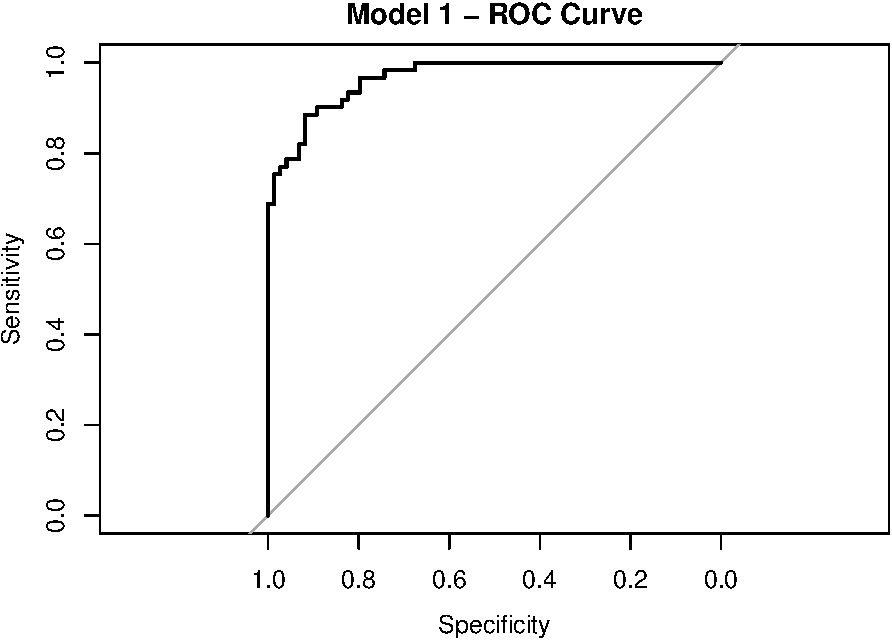
\includegraphics{HW3_Final_files/figure-latex/unnamed-chunk-19-1.pdf}

\begin{verbatim}
## 
## Call:
## roc.formula(formula = factor(target) ~ predict_1, data = testing)
## 
## Data: predict_1 in 74 controls (factor(target) 0) < 61 cases (factor(target) 1).
## Area under the curve: 0.967
\end{verbatim}

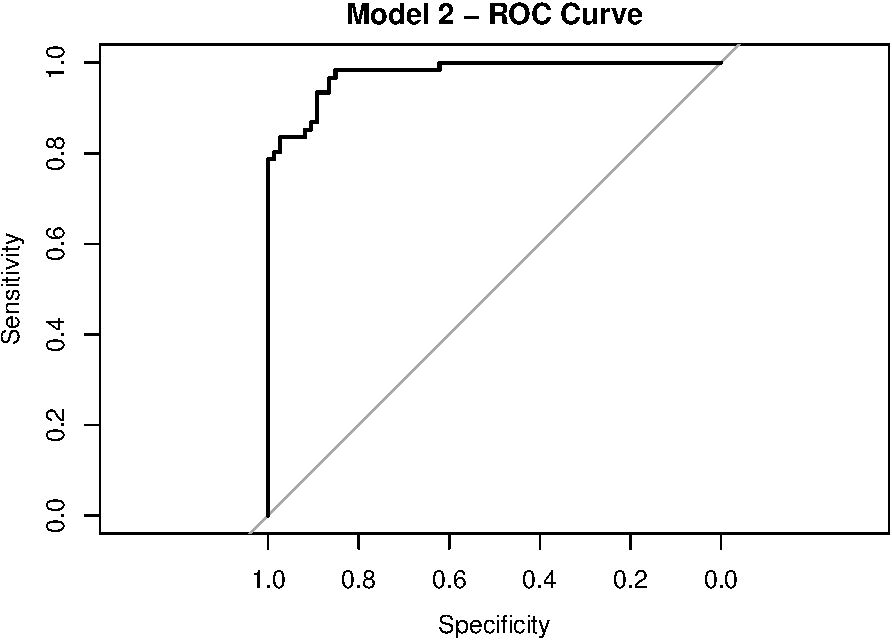
\includegraphics{HW3_Final_files/figure-latex/unnamed-chunk-19-2.pdf}

\begin{verbatim}
## 
## Call:
## roc.formula(formula = factor(target) ~ predict_2, data = testing)
## 
## Data: predict_2 in 74 controls (factor(target) 0) < 61 cases (factor(target) 1).
## Area under the curve: 0.9759
\end{verbatim}

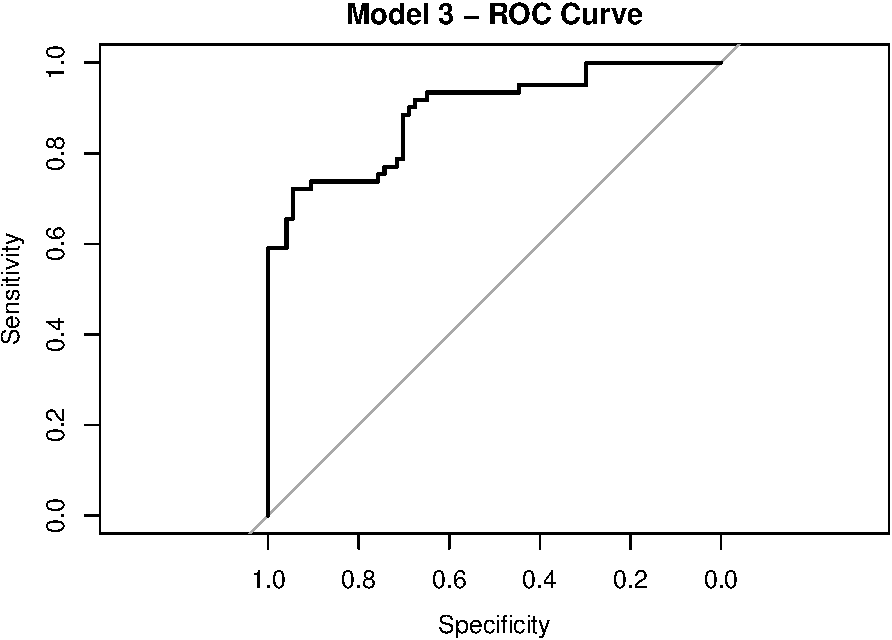
\includegraphics{HW3_Final_files/figure-latex/unnamed-chunk-19-3.pdf}

\begin{verbatim}
## 
## Call:
## roc.formula(formula = factor(target) ~ predict_3, data = testing_pca)
## 
## Data: predict_3 in 74 controls (factor(target) 0) < 61 cases (factor(target) 1).
## Area under the curve: 0.8903
\end{verbatim}

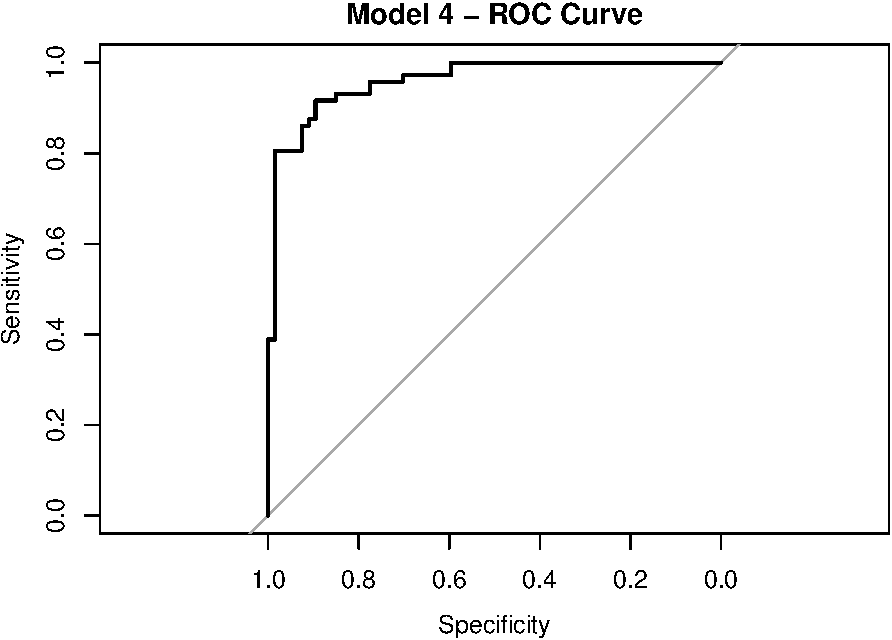
\includegraphics{HW3_Final_files/figure-latex/unnamed-chunk-19-4.pdf}

\begin{verbatim}
## 
## Call:
## roc.formula(formula = factor(target) ~ predict_4, data = testing_norm)
## 
## Data: predict_4 in 67 controls (factor(target) 0) < 72 cases (factor(target) 1).
## Area under the curve: 0.9604
\end{verbatim}

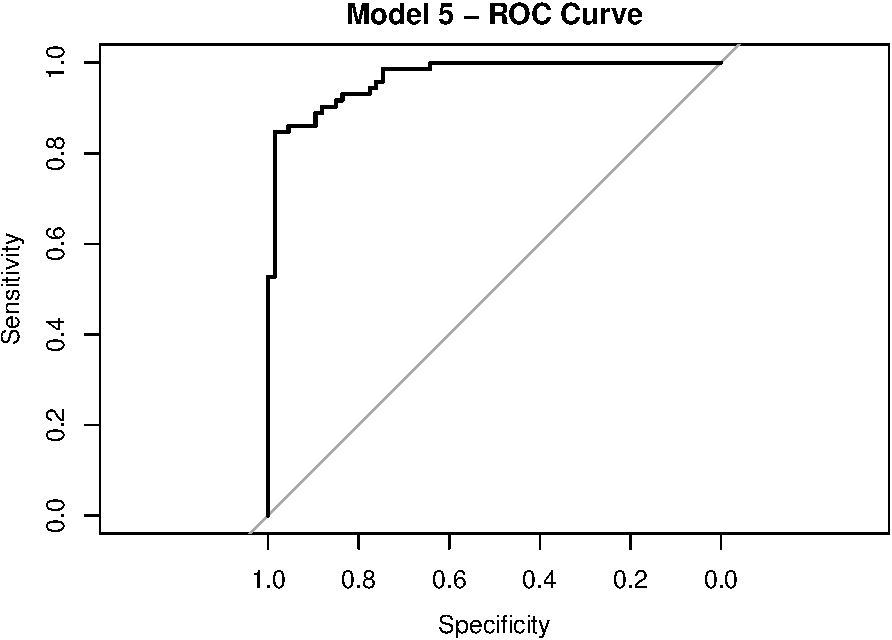
\includegraphics{HW3_Final_files/figure-latex/unnamed-chunk-19-5.pdf}

\begin{verbatim}
## 
## Call:
## roc.formula(formula = factor(target) ~ predict_5, data = testing_norm)
## 
## Data: predict_5 in 67 controls (factor(target) 0) < 72 cases (factor(target) 1).
## Area under the curve: 0.9672
\end{verbatim}

\begin{longtable}[c]{@{}lr@{}}
\caption{Area under the curve}\tabularnewline
\toprule
Model & AUC\tabularnewline
\midrule
\endfirsthead
\toprule
Model & AUC\tabularnewline
\midrule
\endhead
Model 1 & 0.9669916\tabularnewline
Model 2 & 0.9758529\tabularnewline
Model 3 & 0.8903412\tabularnewline
Model 4 & 0.9604063\tabularnewline
Model 5 & 0.9672471\tabularnewline
\bottomrule
\end{longtable}

4 of the 5 area under the curve measurements were above .96, indicating
that all but model 3 have excellent predictive power when measured
against the test set.

\pagebreak

\subsection{Log-likelihood/AIC/BIC}\label{log-likelihoodaicbic}

\begin{longtable}[c]{@{}lrrr@{}}
\caption{Log-likelihood/AIC/BIC}\tabularnewline
\toprule
& Log Likelihood & AIC & BIC\tabularnewline
\midrule
\endfirsthead
\toprule
& Log Likelihood & AIC & BIC\tabularnewline
\midrule
\endhead
Model 1 & -51.49 & 120.98 & 154.81\tabularnewline
Model 2 & -53.51 & 117.01 & 135.81\tabularnewline
Model 3 & -147.25 & 302.49 & 317.53\tabularnewline
Model 4 & -65.67 & 147.34 & 177.66\tabularnewline
Model 5 & -62.45 & 146.91 & 188.60\tabularnewline
\bottomrule
\end{longtable}

Overall, Model 2 stands out with high Accuracy, high Sensitivity, high
Specificity, high AUC, high Log-likelihood number, low AIC and low BIC.
Although Model 3 was the best model to deal with
\textbf{multicollinearity} issues, we still wanted a model with good
prediction.

Model 2 not only greatly minimized the \textbf{multicollinearity} issue,
but also gave the better prediction. We can verify the low level of
multicollinearity in Model 2 by looking at variance inflation factors
(using the `car' library's vif() function. VIF measures how much the
variance of each variable is inflated due to multicollinearity.

\begin{verbatim}
##      nox      tax    lstat     radN 
## 2.009370 1.959690 1.262095 1.970707
\end{verbatim}

Since the scores are all below 4, we can conclude multicollinearity has
been handled appropriately.

More importantly, Likelihood, AIC and BIC numbers also indicate Model 2
is a better model to fit.

\section{Predictions on Evaluation
Data}\label{predictions-on-evaluation-data}

\begin{verbatim}
## 
##  0  1 
## 16 24
\end{verbatim}

After we applied our chosen model (Model 2) to crime-evaluation-data
set, we predicted that for 16 observations \texttt{target} equals 0, and
24 observations, which \texttt{target} equals 1. Please check the file
\emph{result.csv} for detailed information.

\end{document}
